\documentclass[12pt]{article}
\usepackage{amsmath}
\usepackage{graphicx}
\begin{document}
\title{Computer Science M151B, Homework 2}
\date{April 16th, 2018}
\author{Michael Wu\\UID: 404751542}
\maketitle

\section*{Problem 1}

\begin{figure}[ht]
    \begin{center}
        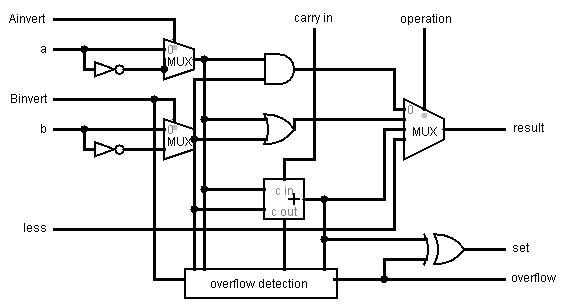
\includegraphics[width=\textwidth]{problem1.png}
    \end{center}
\end{figure}
When overflow has occurred and the highest result bit of the adder is \(0\), this is negative overflow and so we should have \texttt{set}
equal to \(1\). When overflow has occurred and the highest result bit of the adder is \(1\), this is positive overflow and so
we should have \texttt{set} equal to \(0\). Thus doing \(\texttt{overflow} \oplus \texttt{result of adder}\) will produce the correct
\texttt{set} output.

\section*{Problem 2}

Consider the following truth table for the \(1\)-bit adder of the highest bit.
\[\begin{array}{c|c|c|c|c|c}
        A & B & C_\text{in} & C_\text{out} & \text{Result} & \text{Overflow}\\
        \hline
        0 & 0 & 0 & 0 & 0 & 0\\
        0 & 0 & 1 & 0 & 1 & 1\\
        0 & 1 & 0 & 0 & 1 & 0\\
        0 & 1 & 1 & 1 & 0 & 0\\
        1 & 0 & 0 & 0 & 1 & 0\\
        1 & 0 & 1 & 1 & 0 & 0\\
        1 & 1 & 0 & 1 & 0 & 1\\
        1 & 1 & 1 & 1 & 1 & 0
\end{array}\]
Overflow occurs when both inputs \(A\) and \(B\) are \(0\) and the result is \(1\), which corresponds to
the conditions \(A\geq 0\), \(B\geq 0\), and \(\text{Result}<0\). This is the first row in figure 3.2 in the book.
Overflow also occurs when both inputs \(A\) and \(B\) are \(1\) and the result is \(0\), which corresponds to
the conditions \(A<0\), \(B<0\), and \(\text{Result}\geq 0\). This is the second row in figure 3.2 in the book.
Note that in this truth table, \(C_\text{in}\oplus C_\text{out}\) is \(1\) when overflow occurs and \(0\) otherwise.

Now consider implementing subtraction with this adder. In this case, we simply need to invert the bits of one input and add the
inverted number to the other number, along with a carry in. Because our overflow detection works for addition, this should
also detect overflow in subtraction, as all bits will be flipped on one input. For the flipped numbers, the leading bit of a negative
number will become \(0\) and the leading bit of a positive number will become \(1\). So this also implements the same conditions as the
third and fourth rows in figure 3.2 in the book. So overflow will be properly detected in all cases if we use \(C_\text{in}\oplus C_\text{out}\)
as our overflow signal.

\section*{Problem 3}

Because the \texttt{and}, \texttt{or}, and \texttt{nor} operations do not depend on the output of the adder, their results will be the same.
Additionally, the \texttt{add} operation normally has a carry in of \(0\), so it will not be affected either. However, \texttt{sub}
will always output one below the desired result. In the case that the result is supposed to be the most negative integer, \texttt{sub}
will overflow and output the most positive integer instead. Additionally since \texttt{slt} relies on \texttt{sub}, it will return \(1\) for
values that are equal, instead of returning \(0\).

\section*{Problem 4}

We must execute a load word instruction, because this sets \texttt{MemRead} to \(1\) while \texttt{RegDst} is \(0\). If the
load word executes correctly, then we know that \texttt{MemRead} does not become \(0\) when \texttt{RegDst} is \(0\). Let the program
counter be \(0\) and let instruction memory at address \(0\) hold the instruction
\[10001101000010010000000000000000\]
in binary, or equivalently \texttt{lw \$8, 0(\$9)}. Let register \(9\) hold the value \(4\), let register \(8\) hold the value \(0\),
and let data memory hold the word \(1\) at address \(4\). Then after one cycle the load word should be executed, reading memory at address
\(4\) and storing it in register \(8\). If register \(8\) has changed to \(1\) from \(0\), then there is no cross-talk fault between
\texttt{MemRead} and \texttt{RegDst}. If register \(8\) is any other value, then there is a cross-talk fault.

\section*{Problem 5}

The only time that the \texttt{Jump} signal is \(1\) is during a jump instruction. However, the other control signals are don't cares, so
the way that they are set are unknown. They depend on the implementation of the control circuit. For the particular implementation shown
in the book, I will assume that the signal \texttt{RegDst} is \(0\) unless an R-format instruction is being executed. This is supported by
the PLA implementation of the control circuit shown in Appendix D in figure D.2.5. So we must execute a jump instruction to test whether
a cross-talk fault occurs. Let the program counter be \(0\) and let instruction memory at address \(0\) hold the instruction
\[000010 00 0000 0000 0000 0000 0000 0010\]
in binary, or equivalently \texttt{j 2}. Then after one cycle the jump should be executed, making the program counter \(8\). If the
\texttt{Jump} signal is \(0\), then the program counter should increment normally and be \(4\). So if the program counter is \(8\)
we know that there is no cross-talk fault between \texttt{Jump} and \texttt{RegDst}, and if the program counter is \(4\) then we know
that there is a cross-talk fault.

\section*{Problem 6}

These control outputs correspond to \texttt{MemRead} being \(1\), \texttt{RegWrite} being \(1\), and all other control signals being
\texttt{0}. Because both \texttt{Branch} and \texttt{Jump} are \(0\), the program counter will update normally and increment by \(4\).
The format of our instruction is
\begin{center}
\texttt{xxxx xxss ssst tttt xxxx xxxx xxxx xxxx}
\end{center}
where \texttt{s} are the bits input to \texttt{Read register 1}, \texttt{t} are the bits input to \texttt{Read register 2}, and
\texttt{x} are the don't care bits. This is because \texttt{ALUOp} and \texttt{RegDst} are \(0\), so the ALU control unit will not care
about the lowest \(6\) bits and \texttt{RegDst} will choose to use the bits input to \texttt{Read register 2} to input to
\texttt{Write register} as well. Since \texttt{ALUSrc} is \(0\), the data in the register specified by \texttt{Read register 2}
will be chosen along with the data in the register specified by \texttt{Read register 1}. They will be added together since
the \texttt{ALUOp} corresponds to add. The result of this addition will be used as an address and read by the data memory module,
since \texttt{MemRead} is \(1\). However because  \texttt{MemtoReg} is \(0\), we will bypass the data memory read and use the result of
the addition instead. Finally since \texttt{RegWrite} is \(1\), we store the result of the addition into the register specified
by \texttt{Write register}, which is the same register as the one specified by \texttt{Read register 2}.

Overall, over one clock cycle this has the effect of taking the data in the registers given by the \texttt{s} and \texttt{t} bits,
adding them together, then storing the result in the register given by the \texttt{t} bits. Additionally, the program counter is
incremented by \(4\).

\pagebreak

\section*{Problem 7}

No changes are needed to the datapath, we simply need to output new control signals for \texttt{lwrr}. The controls signals
for \texttt{lwrr} should be the same as the control signals for \texttt{lw}, except \texttt{RegDst} should be \(1\) and \texttt{ALUSrc}
should be \(0\). The controls for \texttt{lwrr} are shown in the following table.
\begin{center}
        \begin{tabular} {c|c}
                Signal & Value \\
                \hline
                \texttt{RegDst} & 1\\
                \texttt{ALUSrc} & 0\\
                \texttt{MemtoReg} & 1\\
                \texttt{RegWrite} & 1\\
                \texttt{MemRead} & 1\\
                \texttt{MemWrite} & 0\\
                \texttt{Branch} & 0\\
                \texttt{ALUOp1} & 0\\
                \texttt{ALUOp0} & 0
        \end{tabular}
\end{center}

\pagebreak

\section*{Problem 8}

\paragraph{a)}

\begin{figure}[!ht]
    \begin{center}
        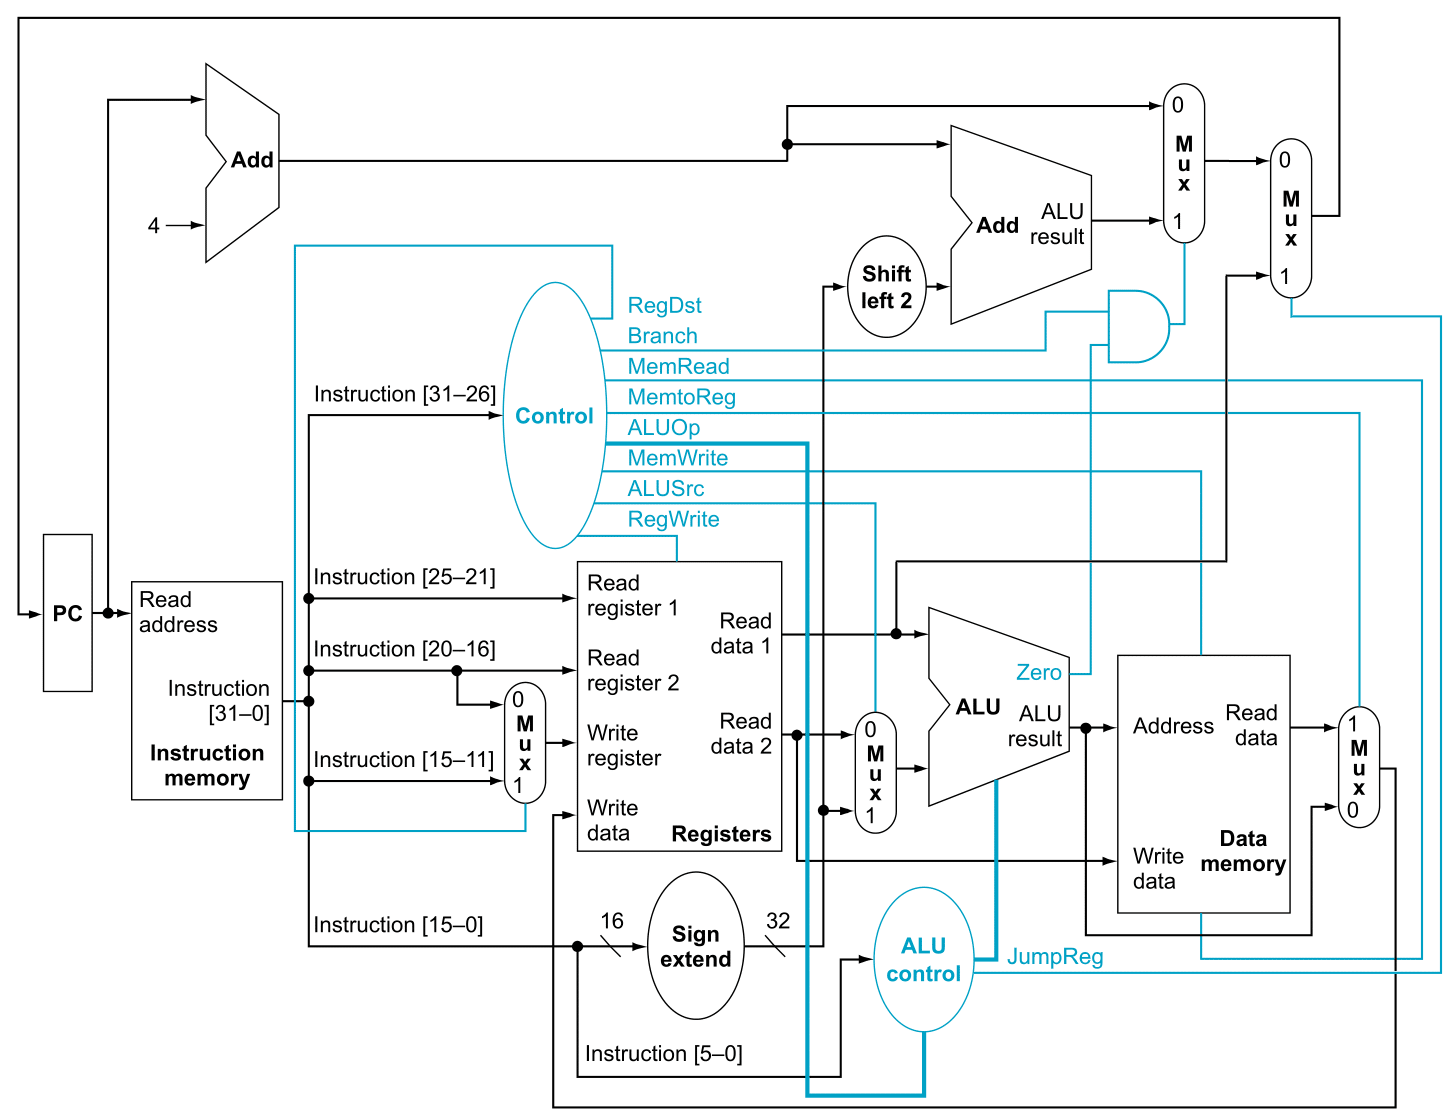
\includegraphics[width=4.4in]{problem8a.png}
    \end{center}
\end{figure}
A new multiplexer is needed to select whether to jump or not. This will come after the branch multiplexer, and will
jump to the data stored in \texttt{Read register 1} if the select is \(1\). The control for this will come
from the \texttt{ALU Control} unit. Since the opcode of \texttt{jr} is \(0\), the \texttt{ALU Control} unit
must check that the \texttt{funct} field is \(8\). If this is the case, it will output \(1\) for the \texttt{JumpReg}
signal, otherwise \texttt{JumpReg} is \(0\).

\paragraph{b)}

A new control signal, \texttt{JumpReg}, must come out of the \texttt{ALU Control} unit. This is \(1\) if the \texttt{funct} field is \(8\)
when \texttt{ALUOp1} is \(1\) and \texttt{ALUOp2} is \(0\), and it is \(0\) otherwise.

\paragraph{c)}

No changes are necessary to the control logic shown in table 4.22, as this is for the main control unit, not the \texttt{ALU Control}
unit. However the signal \texttt{JumpReg} can be implemented by the following logic.
\[\texttt{JumpReg}=\texttt{ALUOp1}\wedge\neg\texttt{ALUOp0}\wedge\neg\texttt{f5}\wedge\neg\texttt{f4}\wedge\texttt{f3}\wedge
\neg\texttt{f2}\wedge\neg\texttt{f1}\wedge\neg\texttt{f0}\]
Here \texttt{f5} to \texttt{f0} denote the bits of the \texttt{funct} field.

\end{document}